
%% bare_jrnl_compsoc.tex
%% V1.3
%% 2007/01/11
%% by Michael Shell
%% See:
%% http://www.michaelshell.org/
%% for current contact information.
%%
%% This is a skeleton file demonstrating the use of IEEEtran.cls
%% (requires IEEEtran.cls version 1.7 or later) with an IEEE Computer
%% Society journal paper.
%%
%% Support sites:
%% http://www.michaelshell.org/tex/ieeetran/
%% http://www.ctan.org/tex-archive/macros/latex/contrib/IEEEtran/
%% and
%% http://www.ieee.org/

%%*************************************************************************
%% Legal Notice:
%% This code is offered as-is without any warranty either expressed or
%% implied; without even the implied warranty of MERCHANTABILITY or
%% FITNESS FOR A PARTICULAR PURPOSE! 
%% User assumes all risk.
%% In no event shall IEEE or any contributor to this code be liable for
%% any damages or losses, including, but not limited to, incidental,
%% consequential, or any other damages, resulting from the use or misuse
%% of any information contained here.
%%
%% All comments are the opinions of their respective authors and are not
%% necessarily endorsed by the IEEE.
%%
%% This work is distributed under the LaTeX Project Public License (LPPL)
%% ( http://www.latex-project.org/ ) version 1.3, and may be freely used,
%% distributed and modified. A copy of the LPPL, version 1.3, is included
%% in the base LaTeX documentation of all distributions of LaTeX released
%% 2003/12/01 or later.
%% Retain all contribution notices and credits.
%% ** Modified files should be clearly indicated as such, including  **
%% ** renaming them and changing author support contact information. **
%%
%% File list of work: IEEEtran.cls, IEEEtran_HOWTO.pdf, bare_adv.tex,
%%                    bare_conf.tex, bare_jrnl.tex, bare_jrnl_compsoc.tex
%%*************************************************************************

% *** Authors should verify (and, if needed, correct) their LaTeX system  ***
% *** with the testflow diagnostic prior to trusting their LaTeX platform ***
% *** with production work. IEEE's font choices can trigger bugs that do  ***
% *** not appear when using other class files.                            ***
% The testflow support page is at:
% http://www.michaelshell.org/tex/testflow/




% Note that the a4paper option is mainly intended so that authors in
% countries using A4 can easily print to A4 and see how their papers will
% look in print - the typesetting of the document will not typically be
% affected with changes in paper size (but the bottom and side margins will).
% Use the testflow package mentioned above to verify correct handling of
% both paper sizes by the user's LaTeX system.
%
% Also note that the "draftcls" or "draftclsnofoot", not "draft", option
% should be used if it is desired that the figures are to be displayed in
% draft mode.
%
% The Computer Society usually requires 10pt for submissions.
%
\documentclass[journal,final,twocolumn,10pt,twoside]{IEEEtranTCOM}
%
% If IEEEtran.cls has not been installed into the LaTeX system files,
% manually specify the path to it like:
% \documentclass[12pt,journal,compsoc]{../sty/IEEEtran}

\usepackage{amssymb}
\usepackage{fixltx2e}
\usepackage{caption}
\usepackage{algorithm}% http://ctan.org/pkg/algorithms
\usepackage[noend]{algpseudocode}% http://ctan.org/pkg/algorithmicx
\makeatletter
\let\OldStatex\Statex
\renewcommand{\Statex}[1][3]{%
  \setlength\@tempdima{\algorithmicindent}%
  \OldStatex\hskip\dimexpr#1\@tempdima\relax}
\makeatother

\newtheorem{lemma}{Lemma}
\newtheorem{defi}[lemma]{Definition}
\newtheorem{observation}{Observation}[section]
\newtheorem{remark}[lemma]{Remark}
\newtheorem{theo}[lemma]{Theorem}
\newtheorem{theorem}[lemma]{Theorem}
\newtheorem{corollary}[lemma]{Corollary}
\newtheorem{defisec}{Definition}[section]
\newtheorem{lemmasec}[defisec]{Lemma}




% Some very useful LaTeX packages include:
% (uncomment the ones you want to load)


% *** MISC UTILITY PACKAGES ***
%
%\usepackage{ifpdf}
% Heiko Oberdiek's ifpdf.sty is very useful if you need conditional
% compilation based on whether the output is pdf or dvi.
% usage:
% \ifpdf
%   % pdf code
% \else
%   % dvi code
% \fi
% The latest version of ifpdf.sty can be obtained from:
% http://www.ctan.org/tex-archive/macros/latex/contrib/oberdiek/
% Also, note that IEEEtran.cls V1.7 and later provides a builtin
% \ifCLASSINFOpdf conditional that works the same way.
% When switching from latex to pdflatex and vice-versa, the compiler may
% have to be run twice to clear warning/error messages.






% *** CITATION PACKAGES ***
%
\ifCLASSOPTIONcompsoc
  % IEEE Computer Society needs nocompress option
  % requires cite.sty v4.0 or later (November 2003)
  % \usepackage[nocompress]{cite}
\else
  % normal IEEE
  % \usepackage{cite}
\fi
% cite.sty was written by Donald Arseneau
% V1.6 and later of IEEEtran pre-defines the format of the cite.sty package
% \cite{} output to follow that of IEEE. Loading the cite package will
% result in citation numbers being automatically sorted and properly
% "compressed/ranged". e.g., [1], [9], [2], [7], [5], [6] without using
% cite.sty will become [1], [2], [5]--[7], [9] using cite.sty. cite.sty's
% \cite will automatically add leading space, if needed. Use cite.sty's
% noadjust option (cite.sty V3.8 and later) if you want to turn this off.
% cite.sty is already installed on most LaTeX systems. Be sure and use
% version 4.0 (2003-05-27) and later if using hyperref.sty. cite.sty does
% not currently provide for hyperlinked citations.
% The latest version can be obtained at:
% http://www.ctan.org/tex-archive/macros/latex/contrib/cite/
% The documentation is contained in the cite.sty file itself.
%
% Note that some packages require special options to format as the Computer
% Society requires. In particular, Computer Society  papers do not use
% compressed citation ranges as is done in typical IEEE papers
% (e.g., [1]-[4]). Instead, they list every citation separately in order
% (e.g., [1], [2], [3], [4]). To get the latter we need to load the cite
% package with the nocompress option which is supported by cite.sty v4.0
% and later. Note also the use of a CLASSOPTION conditional provided by
% IEEEtran.cls V1.7 and later.





% *** GRAPHICS RELATED PACKAGES ***
%
\ifCLASSINFOpdf
  \usepackage[pdftex]{graphicx}
  % declare the path(s) where your graphic files are
  % \graphicspath{{../pdf/}{../jpeg/}}
  % and their extensions so you won't have to specify these with
  % every instance of \includegraphics
  % \DeclareGraphicsExtensions{.pdf,.jpeg,.png}
\else
  % or other class option (dvipsone, dvipdf, if not using dvips). graphicx
  % will default to the driver specified in the system graphics.cfg if no
  % driver is specified.
  % \usepackage[dvips]{graphicx}
  % declare the path(s) where your graphic files are
  % \graphicspath{{../eps/}}
  % and their extensions so you won't have to specify these with
  % every instance of \includegraphics
  % \DeclareGraphicsExtensions{.eps}
\fi
% graphicx was written by David Carlisle and Sebastian Rahtz. It is
% required if you want graphics, photos, etc. graphicx.sty is already
% installed on most LaTeX systems. The latest version and documentation can
% be obtained at: 
% http://www.ctan.org/tex-archive/macros/latex/required/graphics/
% Another good source of documentation is "Using Imported Graphics in
% LaTeX2e" by Keith Reckdahl which can be found as epslatex.ps or
% epslatex.pdf at: http://www.ctan.org/tex-archive/info/
%
% latex, and pdflatex in dvi mode, support graphics in encapsulated
% postscript (.eps) format. pdflatex in pdf mode supports graphics
% in .pdf, .jpeg, .png and .mps (metapost) formats. Users should ensure
% that all non-photo figures use a vector format (.eps, .pdf, .mps) and
% not a bitmapped formats (.jpeg, .png). IEEE frowns on bitmapped formats
% which can result in "jaggedy"/blurry rendering of lines and letters as
% well as large increases in file sizes.
%
% You can find documentation about the pdfTeX application at:
% http://www.tug.org/applications/pdftex





% *** MATH PACKAGES ***
%
\usepackage[cmex10]{amsmath}
% A popular package from the American Mathematical Society that provides
% many useful and powerful commands for dealing with mathematics. If using
% it, be sure to load this package with the cmex10 option to ensure that
% only type 1 fonts will utilized at all point sizes. Without this option,
% it is possible that some math symbols, particularly those within
% footnotes, will be rendered in bitmap form which will result in a
% document that can not be IEEE Xplore compliant!
%
% Also, note that the amsmath package sets \interdisplaylinepenalty to 10000
% thus preventing page breaks from occurring within multiline equations. Use:
%\interdisplaylinepenalty=2500
% after loading amsmath to restore such page breaks as IEEEtran.cls normally
% does. amsmath.sty is already installed on most LaTeX systems. The latest
% version and documentation can be obtained at:
% http://www.ctan.org/tex-archive/macros/latex/required/amslatex/math/





% *** SPECIALIZED LIST PACKAGES ***
%
%\usepackage{algorithmic}
% algorithmic.sty was written by Peter Williams and Rogerio Brito.
% This package provides an algorithmic environment fo describing algorithms.
% You can use the algorithmic environment in-text or within a figure
% environment to provide for a floating algorithm. Do NOT use the algorithm
% floating environment provided by algorithm.sty (by the same authors) or
% algorithm2e.sty (by Christophe Fiorio) as IEEE does not use dedicated
% algorithm float types and packages that provide these will not provide
% correct IEEE style captions. The latest version and documentation of
% algorithmic.sty can be obtained at:
% http://www.ctan.org/tex-archive/macros/latex/contrib/algorithms/
% There is also a support site at:
% http://algorithms.berlios.de/index.html
% Also of interest may be the (relatively newer and more customizable)
% algorithmicx.sty package by Szasz Janos:
% http://www.ctan.org/tex-archive/macros/latex/contrib/algorithmicx/




% *** ALIGNMENT PACKAGES ***
%
%\usepackage{array}
% Frank Mittelbach's and David Carlisle's array.sty patches and improves
% the standard LaTeX2e array and tabular environments to provide better
% appearance and additional user controls. As the default LaTeX2e table
% generation code is lacking to the point of almost being broken with
% respect to the quality of the end results, all users are strongly
% advised to use an enhanced (at the very least that provided by array.sty)
% set of table tools. array.sty is already installed on most systems. The
% latest version and documentation can be obtained at:
% http://www.ctan.org/tex-archive/macros/latex/required/tools/


%\usepackage{mdwmath}
%\usepackage{mdwtab}
% Also highly recommended is Mark Wooding's extremely powerful MDW tools,
% especially mdwmath.sty and mdwtab.sty which are used to format equations
% and tables, respectively. The MDWtools set is already installed on most
% LaTeX systems. The lastest version and documentation is available at:
% http://www.ctan.org/tex-archive/macros/latex/contrib/mdwtools/


% IEEEtran contains the IEEEeqnarray family of commands that can be used to
% generate multiline equations as well as matrices, tables, etc., of high
% quality.


%\usepackage{eqparbox}
% Also of notable interest is Scott Pakin's eqparbox package for creating
% (automatically sized) equal width boxes - aka "natural width parboxes".
% Available at:
% http://www.ctan.org/tex-archive/macros/latex/contrib/eqparbox/





% *** SUBFIGURE PACKAGES ***
%\ifCLASSOPTIONcompsoc
%\usepackage[tight,normalsize,sf,SF]{subfigure}
%\else
%\usepackage[tight,footnotesize]{subfigure}
%\fi
% subfigure.sty was written by Steven Douglas Cochran. This package makes it
% easy to put subfigures in your figures. e.g., "Figure 1a and 1b". For IEEE
% work, it is a good idea to load it with the tight package option to reduce
% the amount of white space around the subfigures. Computer Society papers
% use a larger font and \sffamily font for their captions, hence the
% additional options needed under compsoc mode. subfigure.sty is already
% installed on most LaTeX systems. The latest version and documentation can
% be obtained at:
% http://www.ctan.org/tex-archive/obsolete/macros/latex/contrib/subfigure/
% subfigure.sty has been superceeded by subfig.sty.


%\ifCLASSOPTIONcompsoc
%  \usepackage[caption=false]{caption}
%  \usepackage[font=normalsize,labelfont=sf,textfont=sf]{subfig}
%\else
%  \usepackage[caption=false]{caption}
%  \usepackage[font=footnotesize]{subfig}
%\fi
% subfig.sty, also written by Steven Douglas Cochran, is the modern
% replacement for subfigure.sty. However, subfig.sty requires and
% automatically loads Axel Sommerfeldt's caption.sty which will override
% IEEEtran.cls handling of captions and this will result in nonIEEE style
% figure/table captions. To prevent this problem, be sure and preload
% caption.sty with its "caption=false" package option. This is will preserve
% IEEEtran.cls handing of captions. Version 1.3 (2005/06/28) and later 
% (recommended due to many improvements over 1.2) of subfig.sty supports
% the caption=false option directly:
%\ifCLASSOPTIONcompsoc
%  \usepackage[caption=false,font=normalsize,labelfont=sf,textfont=sf]{subfig}
%\else
%  \usepackage[caption=false,font=footnotesize]{subfig}
%\fi
%
% The latest version and documentation can be obtained at:
% http://www.ctan.org/tex-archive/macros/latex/contrib/subfig/
% The latest version and documentation of caption.sty can be obtained at:
% http://www.ctan.org/tex-archive/macros/latex/contrib/caption/




% *** FLOAT PACKAGES ***
%
\usepackage{fixltx2e}
\usepackage{subfigure}

\usepackage{dblfloatfix}% http://ctan.org/pkg/dblfloatfix
\usepackage{lipsum}% http://ctan.org/pkg/lipsum

\hyphenation{op-tical net-works semi-conduc-tor}


\begin{document}
\title{Converting a network into a small-world network: 
A fast algorithm for minimizing average path length through link addition}    


%\author{A. Author, B. Author
%\thanks{}}

% note the % following the last \IEEEmembership and also \thanks - 
% these prevent an unwanted space from occurring between the last author name
% and the end of the author line. i.e., if you had this:
% 
% \author{....lastname \thanks{...} \thanks{...} }
%                     ^------------^------------^----Do not want these spaces!
%
% a space would be appended to the last name and could cause every name on that
% line to be shifted left slightly. This is one of those "LaTeX things". For
% instance, "\textbf{A} \textbf{B}" will typeset as "A B" not "AB". To get
% "AB" then you have to do: "\textbf{A}\textbf{B}"
% \thanks is no different in this regard, so shield the last } of each \thanks
% that ends a line with a % and do not let a space in before the next \thanks.
% Spaces after \IEEEmembership other than the last one are OK (and needed) as
% you are supposed to have spaces between the names. For what it is worth,
% this is a minor point as most people would not even notice if the said evil
% space somehow managed to creep in.


\maketitle
% The paper headers

\begin{abstract}
The average path length in a network is an important parameter for measuring the 
end-to-end delay for message delivery. The delay between an arbitrary pair of nodes 
is smaller if the average path length is low. It is possible to reduce the average
path length of a network by adding one or more additional links between pairs of nodes.
However, a na\"ive algorithm is often very expensive for determining which additional link 
can reduce the average path length in a network the most. In this paper, we present 
an efficient algorithm to minimize the average network path length by link addition.  
Our algorithm can process significantly larger networks compared to the na\"ive 
algorithm. We present a simple implementation of our algorithm, as well as a performance 
study of it in this paper.  
\end{abstract}


\section{Introduction}
Many real-world networks are modeled as a graph, $G=(V,E)$, where $V$ is a set of vertices  
and $E$ is a set of edges connecting some of the vertex pairs from the set $V$. Any message sent 
from a source to a destination propagates through intermediate vertices.  
A packet incurs {\em end-to-end delay} if it has to go through many 
intermediate hops. Since any pair of nodes can act as a source-destination pair, it is desirable 
that all paths in a network go through as few intermediate hops as possible. In other words, 
any traffic in the network will incur less average delay if the average path length 
in the network is low. Quite often the edges of these graphs are considered to be weighted, 
the weights may indicate the cost of establishing an edge, the latency or other factors 
depending on the context of the network.  

Many networks have regular structures, meaning each node is connected to an equal number 
of nodes on an average. This makes the average path lengths in real-world networks quite long. 
In {\em small-world} networks the degree distribution of the nodes follows a power law 
and the average distance between any pair of nodes is usually small. These networks are of  
interest for quite sometime since Milgram's pioneering paper \cite{M}. Watts and Strogatz \cite{WS}
designed an approach that improves the clustering coefficient of a random network and converts 
a random network into a small-world network. Comellas and Sampels \cite{CS} replaced each node of a 
network by a mesh network, the number of nodes in the mesh is equal to the 
degree of the node that is replaced
by the mesh. This converted an arbitrary network into a small-world network. Fall \cite{F} showed that 
the addition of a few random edges in a network can reduce the average path length of a network 
significantly. Lu {\em et al.} \cite{LSG} showed that an arbitrary network can be made into a 
small-world network by introducing a scale-free distribution of nodes in a binary tree network.
 

The small-world nature of a network can be characterized in several different ways. 
However, our focus in this article is the average path length for all pairs of nodes.  
Usually a lower average 
path length reduces the overall communication cost in a network. 
Though there is strong evidence from previous work by Fall ~\cite{F} that addition of extra 
edges can reduce the average path length in a network, the algorithmic nature of this problem 
has been studied only recently. 

Meyerson and Tagiku \cite{MT} have shown that the general problem of adding $k$ edges for minimizing 
the weighted average shortest path lengths between all pairs of vertices is NP-complete. They designed 
several approximation algorithms for this problem \cite{MT}. We are 
interested in this paper in designing an algorithm that adds a single edge to an existing network 
for minimizing the average shortest path lengths between every pair of vertices. Though it may 
seem quite a restricted problem, it has applications in many different areas. Chang {\em et al.}
\cite{CCKN,CSTC} have considered the problem of adding radio-frequency (RF) links in multi-core processor 
design. Their aim is to reduce the latency of communication in multi-core architectures, by adding 
extra radio frequency links on top of a regular interconnection scheme like a mesh network. However 
RF interconnects require much more area and cannot replace the traditional interconnects. Adding even 
a single RF interconnect can improve latency significantly \cite{CCKN,CSTC}. The weight on 
the link is the area requirement for an RF interconnect in this case. Ogras and Marculescu \cite{OM} 
consider a long range link over a regular mesh network for designing efficient Network-on-Chip (NoC) 
in VLSI design. The length of the long link and the volume of traffic between the nodes are  the weights 
on the links in this case. Pickavet and Demeester 
\cite{PD} have designed heuristic algorithms for link restoration in Synchronous Digital Hierarchy (SDH)
networks. One of the key parts in their four-phase algorithm is local optimization, where they 
try to improve the topology in terms of the spare capacity, by adding an extra link. The weight 
on the link is the spare capacity in this case. Jin {\em et al.} \cite{JGN} and Newman \cite{N} 
have simulated stronger community structures in artificial social networks by link addition. It 
is possible to strengthen a community by adding an extra link between two nodes $v_i$ and $v_j$ 
such that they share a relatively large number of friends. The probability of a link addition 
is the weight on an edge in this case and the probability is determined by counting the number of common 
friends.     

Recently Gaur {\em et al.} ~\cite{GCM} have studied several deterministic link addition strategies 
for converting an arbitrary unweighted and undirected network into a small-world network. They found that 
the best strategy is  
to add an additional (long) link in an arbitrary network to minimize 
the average path length of the network. 
Given a graph $G=(V,E)$, 
Gaur {\em et al.} \cite{GCM} considers an $O(V^2\log V)$ algorithm for the all-pairs 
shortest path algorithm for unweighted and undirected graphs. This algorithm is based 
on Dijkstra's shortest path algorithm and not an original contribution by Gaur {\em et al.} as 
they have stated explicitly in their paper \cite{GCM}. 
There is a possibility of introducing 
$O(V^2)$ new edges in a connected graph. The all-pairs shortest path 
algorithm is run after introducing each new edge and the average path length is computed. 
Hence the all-pairs shortest path algorithm needs to be run $O(V^2)$ time and the overall 
complexity of determining which link addition results in the minimum average path length is 
$O(V^2\times V^2\log V)=O(V^4\log V)$. 

In this paper we present a more efficient algorithm for the problem of introducing a new link 
for minimizing the average path length. Our algorithm, unlike that considered by 
Gaur {\em et al.} \cite{GCM}, works on weighted, directed graphs, when the weights 
are non-negative. Hence the complexity of our algorithm is asymptotically strictly better than 
the algorithm considered by Gaur {\em et al.}\cite{GCM}. We present our algorithm, its time complexity and also 
experimental results in this paper. Our algorithm runs in $O(V^2E+V^3)$ time, which has a 
worst-case time complexity of $O(V^4)$ as opposed to the na\"ive algorithm that takes $O(V^5)$
time for weighted directed graphs.   

\section{An efficient algorithm for link addition that minimizes the average path length}

In general, the shortest path between vertices $v_i$ and $v_j$ is the path that has the minimum sum weight. 
In the simplest case each edge has a unit weight, or is unweighted, and the shortest path is the minimum 
number of edges between $v_i$ and $v_j$. 
The {\em single-source shortest path} (SSSP) algorithm finds the shortest paths between a given 
vertex $v_i$ and 
all other vertices in the graph; and the {\em all-pairs shortest path} (APSP) algorithm finds the shortest paths 
between all pairs of vertices. We refer the reader to the book by Cormen {\em et al.}\cite{CLRS} for a review of 
shortest path algorithms. 
We will use the Floyd-Warshall algorithm as the basis of our new algorithm, as it is known to be one of the most 
efficient algorithms for this problem \cite{CLRS}. 
We refer to the problem of {\em link addition that minimizes the average path length} as the {\em MinAPL} problem 
as in ~\cite{GCM}. A na\"ive application of the Floyd-Warshall algorithm can solve this problem in the following way. 
We first compute the APSP of a graph $G$ by executing the Floyd-Warshall algorithm in $O(V^3)$ time, and compute the 
average path length of $G$. Next, we introduce all possible $O(V^2)$ additional links and compute the average 
path length of the resulting graph by using the Floyd-Warshall algorithm and determine the link whose addition 
minimizes the average path length. This algorithm will take $O(V^2\times V^3)=O(V^5)$ time. We show in this 
paper that it is possible to solve this problem in $O(V^4)$ time resulting in a much faster algorithm. 

algor


We have done extensive experiments for evaluating the performance of our algorithm. All experiments 
were run on a Virtualbox Ubuntu 14.04 on an i7 3630QM processor.  The algorithm was implemented using C++ and the GNU C++ compiler. 
For each of the experiments we have ensured that the output of our algorithm matches the output from the 
na\"ive algorithm exactly. 
All our graphs were generated through random introduction 
of edges ensuring that the graph was connected. First we generated random graphs with $40$ vertices 
with different edge densities as a fraction of the total possible edges of the complete graph. The set of augmenting edges was defined as the remaining edges not added to the graph. The 
performance comparison of the na\"ive algorithm with our algorithm is shown in Figure \ref{fig1}. The weights 
on the edges are randomly generated with a value between $1$ and $100$.
Our algorithm runs much faster for 
both sparse and dense graphs. If the total number of edges for the complete graph is represented as 
$C$, our algorithm runs in less than a milliseconds for $0.3C$ augmenting edges, while the na\"ive algorithm 
runs in about 38 milliseconds. Similarly, for $0.7C$ augmenting edges, our algorithm runs in $2.3$ milliseconds, 
whereas the na\"ive algorithm takes over $100$ milliseconds. Though we have run our algorithm several times for 
each graph, the running times were almost identical for each run and hence we have not shown any confidence intervals 
in the graphs.  

Next, we evaluated the run times of the two algorithms for larger graphs. We fixed the number of augmenting edges to $0.4C$ while increasing the 
number of vertices. The results are shown for the na\"ive algorithm 
and our algorithm in Figure \ref{fig2}. Our algorithm outperforms 
the na\"ive algorithm significantly in this case as well. For example, the runtime of the two algorithms 
are $46.54$ and $4472.14$ milliseconds respectively for a graph with $100$ vertices. Similarly, for 
a graph with $400$ vertices, the respective runtimes are $11873.8$ and $4.18\times 10^6$ milliseconds 
respectively. 

We also evaluated the performance of our algorithm in terms of the improvement in the average shortest paths after addition of 
a link, as shown in Fig. \ref{fig3}. The weights on the edges were generated randomly and each weight is a number between 
$1$ and $100$. The density of the edges in each graph was $0.6C$ and the augmenting edge was chosen each time from the remaining 
$0.4C$ of the edges. Each data point is an average of $10$ independent runs and the error bars indicate the standard deviation 
on either side of the average. 

\begin{figure}[!t]
\centering
\includegraphics[scale=1.0, width=\columnwidth]{third.pdf}
\vspace{-4cm}
\caption{The performance comparison between our algorithm and the na\"ive algorithm for different
         graph sizes. Each graph has a fraction of $0.6$ of the total edges. The augmenting edge is
         chosen from the remaining fraction of $0.4$ of the total edges. The runtime is plotted
         in a logarithmic scale.}
\label{fig2}
\end{figure}


\begin{figure}
\centering
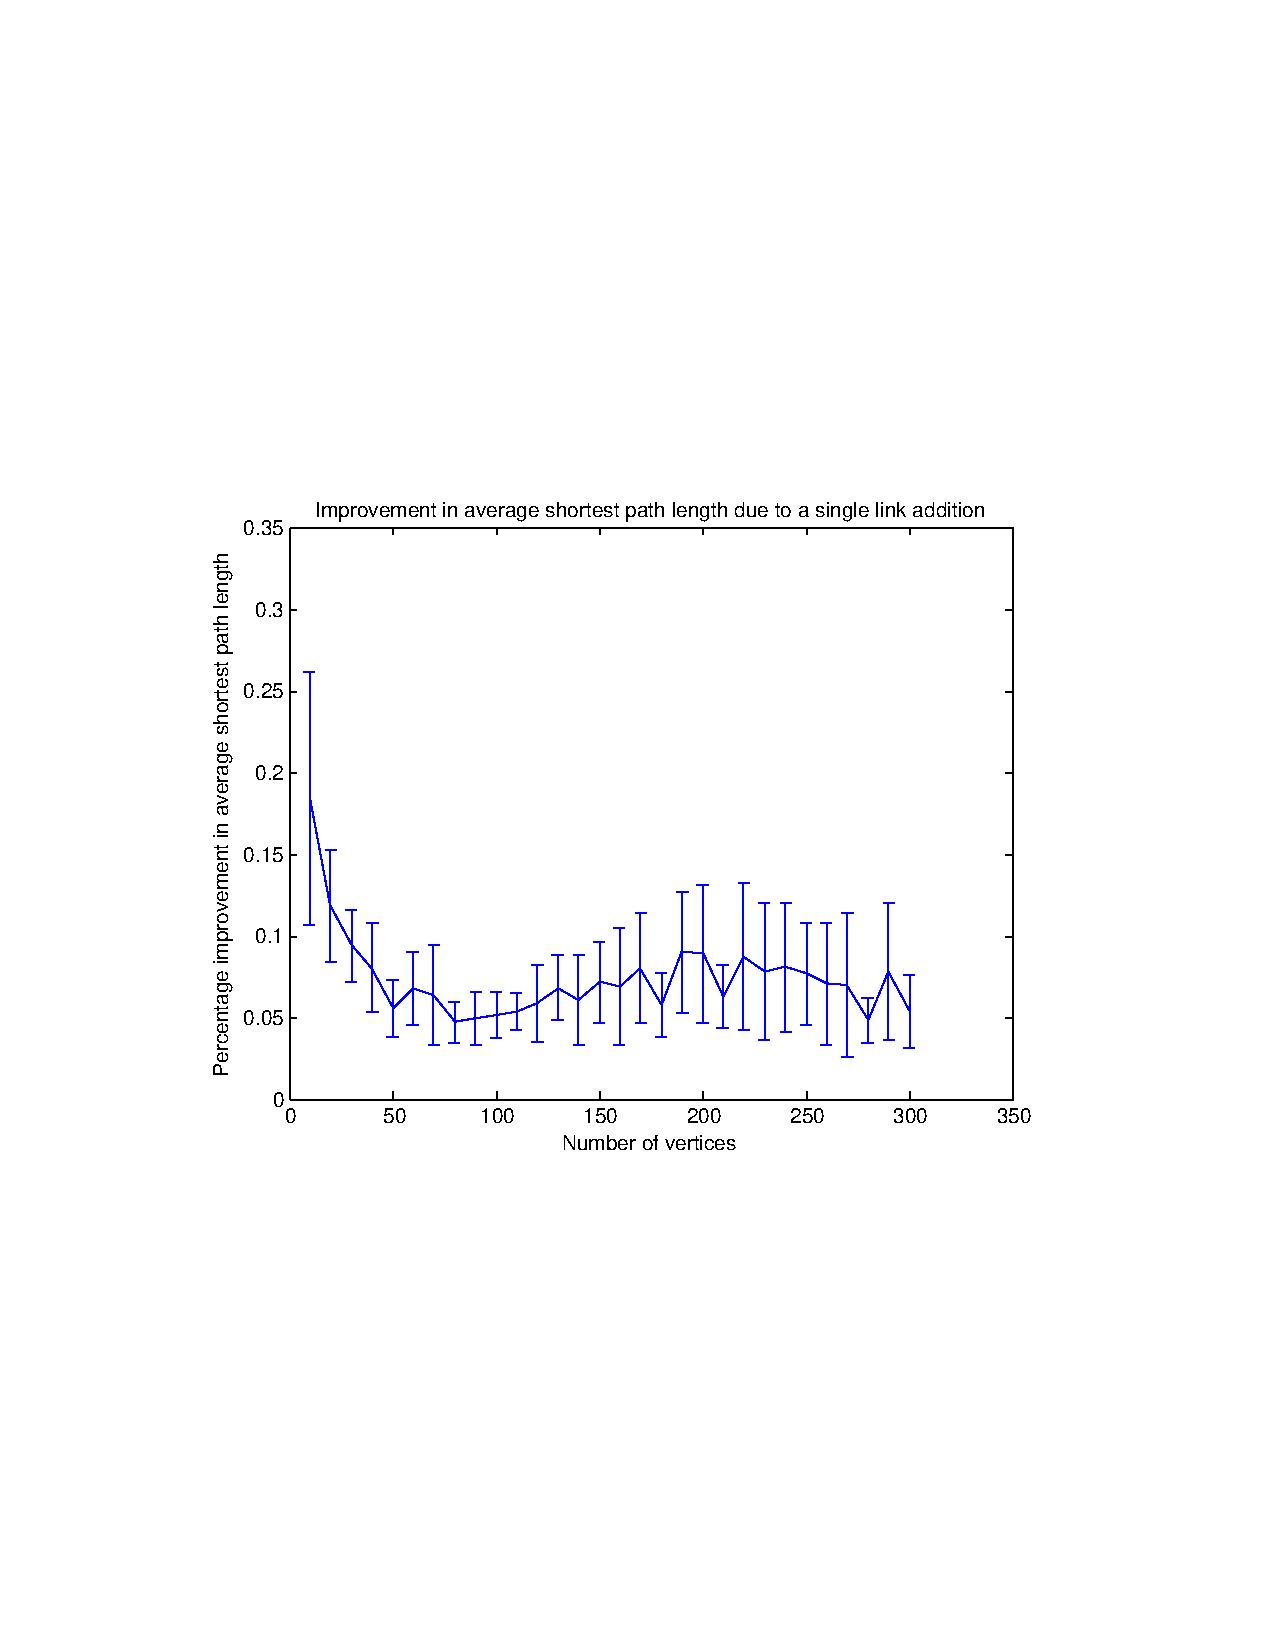
\includegraphics[scale=1.0, width=\columnwidth]{first.pdf}
\vspace{-4cm}
\caption{This graph shows the improvement in average shortest path length due to the addition of a
         single edge. All the graphs contain a fraction of $0.6$ of all possible edges. The
         augmenting edge is chosen randomly from the remaining fraction of $0.4$ of the edges. The
         weights on the edges were randomly generated. The error bars show the standard deviation for
         $10$ runs for each graph.}
\label{fig3}
\end{figure}

\section{Conclusion}

We have presented a simple and efficient algorithm for adding an edge in a graph for minimizing the average shortest path length of the graph. The algorithm improves upon the na\"ive algorithm significantly and can be used 
for addition of edges in large graphs for minimizing the average path length. As an example, our algorithm 
finds an augmenting edge that minimizes the average path length of a graph with $1000$ vertices in about 
$7$ minutes.   

\section{Acknowledgments}

The authors would like to thank the two anonymous reviewers for their extensive comments that helped us to improve the 
presentation of the paper considerably. 

\begin{thebibliography}{1}

\bibitem{CS}
F. Comellas and M. Sampels, ``Deterministic small-world networks", 
{\em Phys. A, Stat. Mech. Appl.}, Vol. 309, No.1 , pp. 231-235, June 2002. 

\bibitem{CLRS}

T. Cormen, C. Leiserson, R. Rivest and C. Stein, {\em Introduction to Algorithms}, 
 MIT Press, Cambridge, MA, 2001. 

\bibitem{CCKN}
M. Frank Chang, J. Cong, A. Kaplan, M. Naik, G. Reinman, E. Socher and 
S-W. Tam,
``CMP Network-on-Chip overlaid with multi-band RF-interconnect"
{\em Proc. International Symposium on High Performance Computer Architecture},
pp. 191-202, 2008. 

\bibitem{CSTC}
M. Frank Chang, E. Socher, S-W. Tam, J. Cong and G. Reinman, 
``RF interconnects for communications on-chip", 
{\em Proc. 2008 International Symposium on Physical Design}, 
pp. 78-83, ACM, 2008.  

\bibitem{F}
K. Fall, ``A delay-tolerant network architecture for challenged Internets", 
{\em Proc. ACM SIGCOMM}, pp. 27-34, August 2003. 

\bibitem{GCM}
N. Gaur, A. Chakraborty and B.S. Manoj,
``Delay optimized small-world networks",
{\em IEEE Communications Letters}, Vol. 18, No. 11, pp. 1939-1942, November 2014.

\bibitem{JGN}
E. M. Jin, M. Girvan and M. Newman, 
``The structure of growing social networks",
{\em Santa Fe Institute Working Paper}, 2001-06-032, 2001. 

\bibitem{M}
S. Milgram, ``The small-world problem", {\em Psychology Today}, Vol. 1, No. 1, 
pp. 61-67, May 1967. 

\bibitem{MT}
A. Meyerson and B. Tagiku, ``Minimizing average shortest path distances via shorcut edge
addition", {Proc. 13th International Workshop on Approximation, Randomization and Combinatorial
Optimization}, LNCS. Vol. 5687, pp. 272-285, 2009.

\bibitem{N}
M. Newman,
``The structure and function of complex networks",
{\em SIAM Review}, Vol. 45, No. 2, pp.167-256, 2003. 


\bibitem{NW} M. Newman and D. Watts, ``Renormalization group analysis of the
small-world network model", {\em Phys. Lett. A}, Vol. 263, No. 4-6, pp. 341-346, December 1999.

\bibitem{OM}
U. Ogras and R. Marculescu,
````It's a small world after all": NoC performance optimization via long-range 
link insertion", {\em IEEE Transactions on Very Large Scale Integration (VLSI) 
Systems}, Vol. 14, No. 7, pp. 693-706, 2006. 

\bibitem{PD}
M. Pickavet and P. Demeester,
``A zoom-in approach to design SDH mesh restorable networks",
{\em Journal of Heuristics}, Vol. 6, pp. 107-130, 2000.

\bibitem{WS}
D. Watts and S. Strogatz,
``Collective dynamics of small-world network", {\em Nature}, Vol. 393, No. 6684, pp. 440-442, June 1998. 

\bibitem{LSG}
Z. Lu, Y. Su and S. Guo, 
``Deterministic scale-free small world networks of arbitrary order", 
{\em Phys. A, Stat. Mech. Appl.}, Vol. 392, No. 17, pp. 3555-3562, April 2013. 

\end{thebibliography}

\end{document}


